\documentclass{article}
\usepackage[left=35mm,top=26mm,right=26mm,bottom=15mm]{geometry}
\usepackage[utf8]{inputenc}
\usepackage{array}
\usepackage{amsmath}
\usepackage{graphicx}
\title{\Huge AE 227 Assignment 5}
\author{\Huge Krishna Wadhwani-160010031 }
\date{November 2017}

\begin{document}

\maketitle

\section{Question 1}

To find the centroid of the give figure, I divide the figure into 4 rectangles and calculate the centroid of the given figure from the centroids of the 4 rectangles.\\

\begin{center}


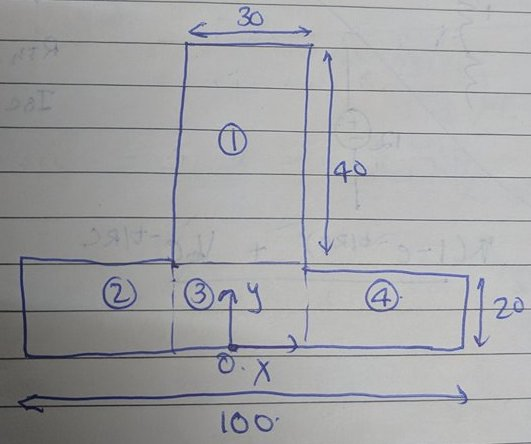
\includegraphics[scale=0.25]{Q!.jpg}
\bigbreak
\begin{tabular}{ | m{1cm} | m{1cm}| m{1cm} | m{1cm} | m{1cm}| m{1cm}| } 
\hline
 $i$ & $A_i$ & $x_i$ & $y_i$ & $A_ix_i$ & $A_iy_i$\\ 
\hline
1 & 12 & 0 & 4 & 0 & 48 \\ 
\hline
2 & 7 & $-$3.25 & 1 & $-$21.75 & 7 \\  
\hline
3 & 6 & 0 & 1 & 0 & 6 \\ 
\hline
4 & 7 & 3.25 & 1 & 21.75 & 7 \\ 
\hline
\end{tabular}
\end{center}

\noindent For the coordinates of centroid($\overline{x},\overline{y} $): \\
$\overline{x} =\dfrac{\sum_i A_ix_i}{\sum_i A_i}$ \ \ \ $\overline{y} =\dfrac{\sum_i A_iy_i}{\sum_i A_i}$\\

\noindent Using values from the above table we get:\\ 

\noindent$\sum_i A_i= 12+7+7+6= 32 cm^2$\\

\noindent $\overline{x} = \dfrac{0-21.75+0+21.75}{32}$\\
$\implies \overline{x} = 0$\\

\noindent $\overline{y} = \dfrac{48+7+6+7}{32}$
\\ 

\noindent$\implies \overline{y} = 2.125 \ cm$\\

\noindent So, centroid ($\overline{x},\overline{y} $) =($0,2.125 $)\\

\noindent \underline{Moment of Inertia}

\noindent $ I_{xy}= \int xydA$\\
As the given figure is symmetric about y-axis, $I_{xy}=0$ as integrant is an odd function in $x$.\\

\noindent For calculation of $I_{xx}, I_{yy}$ and $I_{zz}$, I divide the figure into 2 rectangles(combining rectangles 2,3 and 4 as rectangle 2) and calculate the moment of inertia of the 2 rectangles about their respective centroids.\\

\noindent For rectangle 1 [centorid $c_1=(0,1)$]-\\
$I_{xx1}=\int y^2dA$\\
$\implies I_{xx1}=\dfrac{b_fh_f^3}{12}$\\
$\implies I_{xx1}=6.667\ cm^4$\\

\noindent $I_{yy1}=\int x^2dA$\\
$\implies I_{yy1}=\dfrac{b_f^3h_f}{12}$\\
$\implies I_{xx1}=166.667\ cm^4$\\

\noindent For rectangle 2 [centorid $c_2=(0,4)$]-\\
$I_{xx2}= \dfrac{b_wh_w^3}{12}$\\
$\implies I_{xx2}= 16\ cm^4$\\
$ I_{yy2}=\dfrac{b_w^3h_w}{12} $\\
$\implies I_{yy2}= 9\ cm^4$

\noindent For the moment of inertia of the overall figure about an axis perpendicular to the plane, I will use parallel-axis theorem.\\

\noindent $I_{xx}=(I_{xx1}+A_1d_{1x}^2) +(I_{xx2}+A_2d_{2x}^2)$\\
where $d_{ij}$ is the distance between the centroid of the overall figure and centroid of the $i$th rectangle measured along the axis perpendicular to $j$. It is the distance between axes parallel to $j$ and passing through centroid of the overall figure and centroid of $ith$ rectangle \\
$d_1x=4-2.125= 1.875 \ cm$\\
$d_2x=2.125-1= 1.125 \ cm$\\
$d_1y=0 \ cm$\\
$d_2y=0 \ cm$\\
$A_1= 12 \ cm^2$\\
$A_2= 20 \ cm^2$\\

\noindent Using these values, we get: \\
$\implies I_{xx} = 90.17\ cm^4$\\
$\implies I_{xx} = 175.67\ cm^4$\\

\noindent Using perpendicular axis theorem, we get $I_{zz}$ as:\\
$I_{zz}=I_{xx}+I_{yy}$\\
$\implies I_{zz}= 265.84\ cm^4$

 


\newpage

\section{Question 2}

To find the centroid of the give figure, I divide the figure into rectangles and triangles.\\
\begin{center}
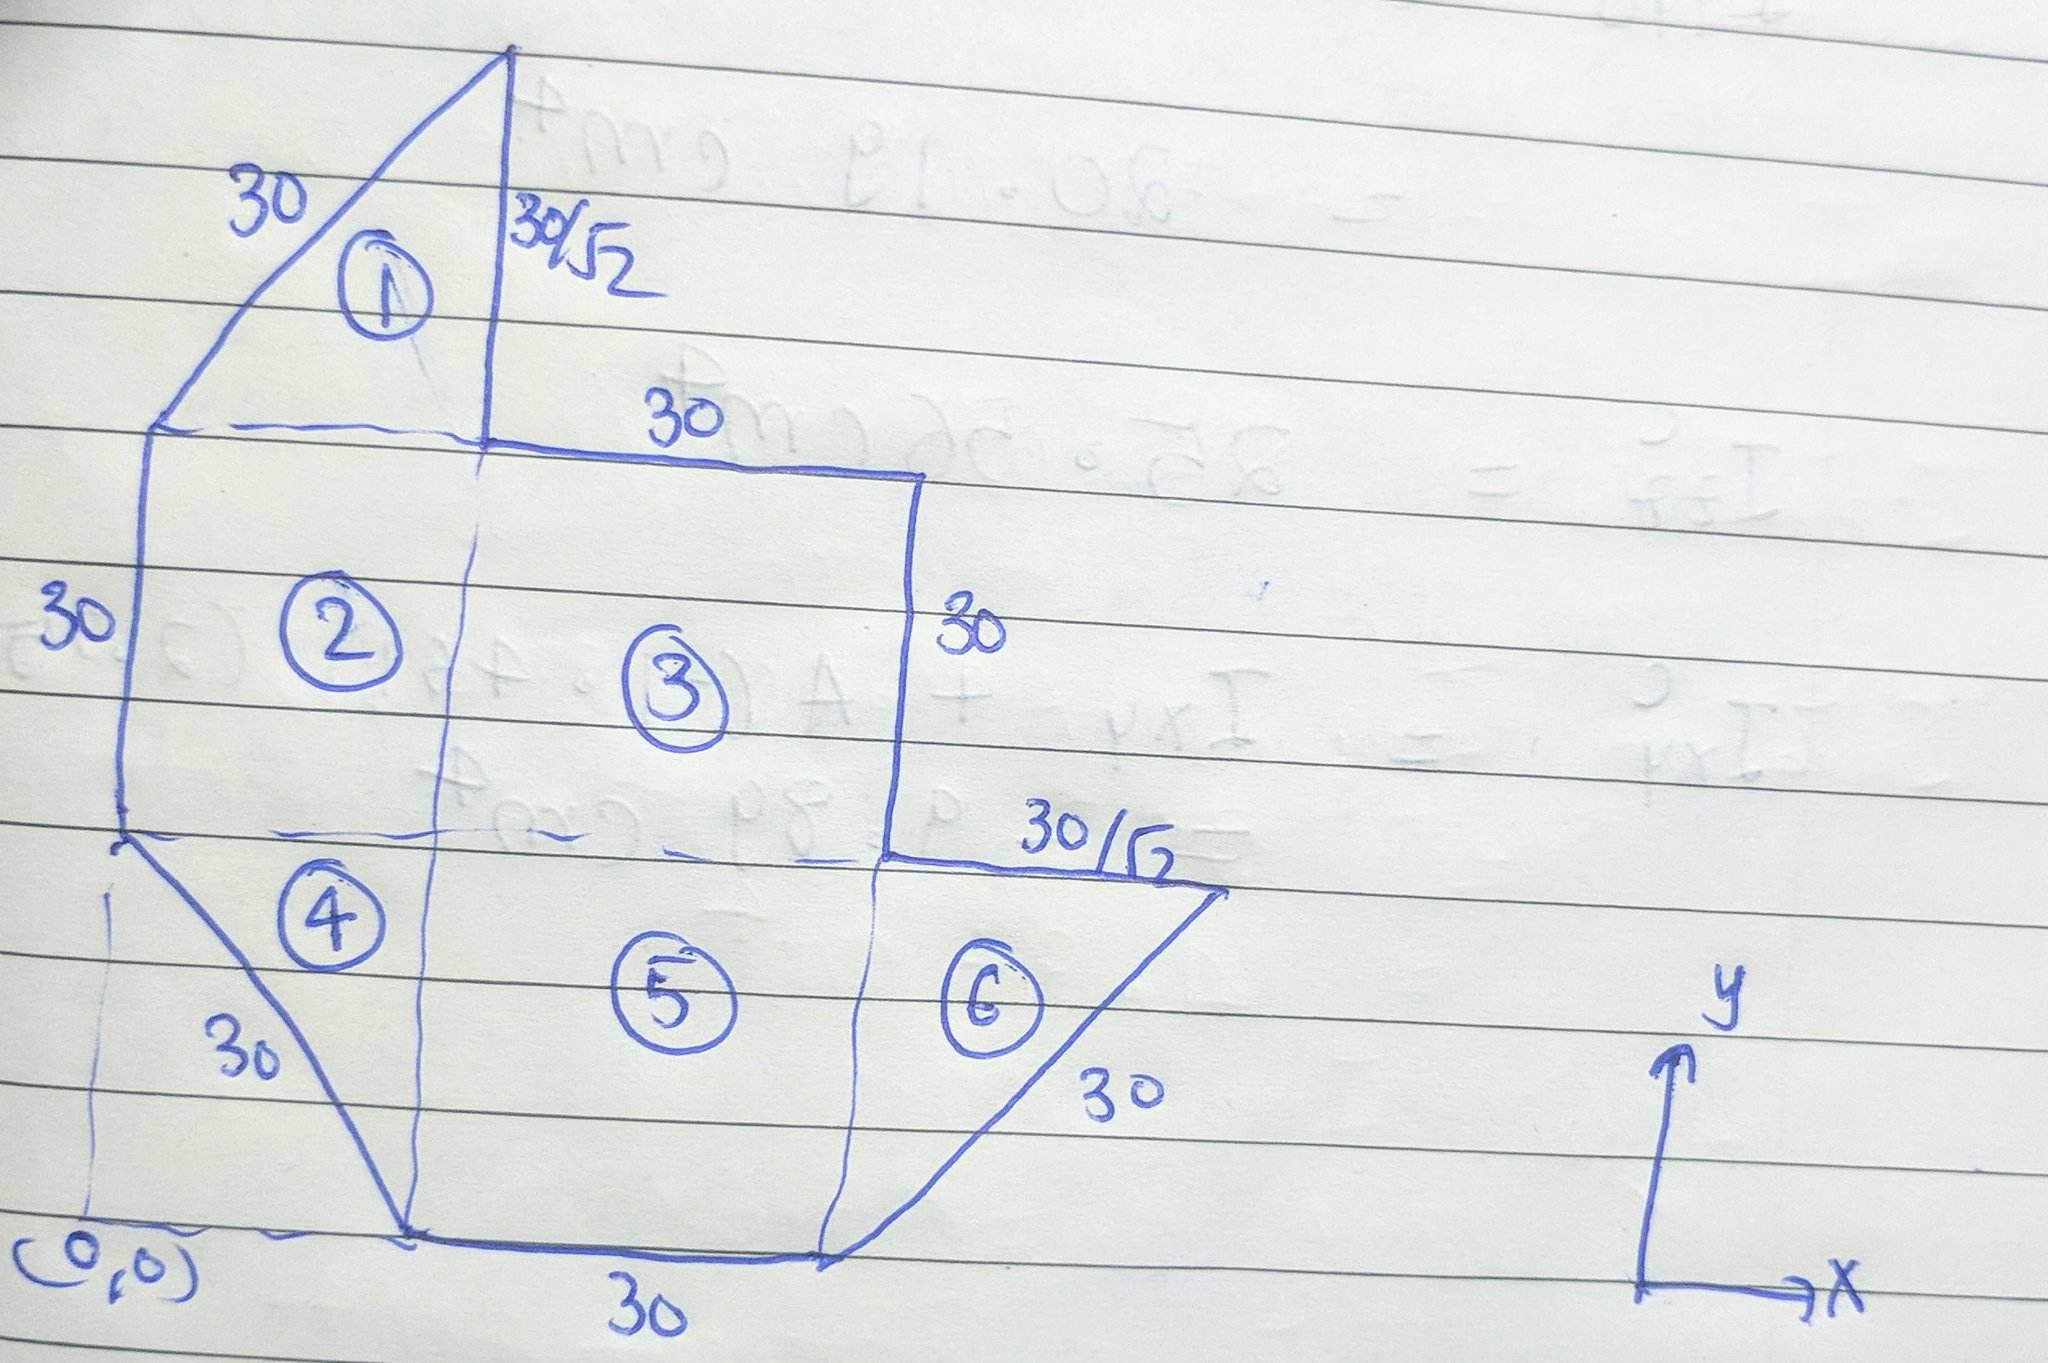
\includegraphics[scale=0.1]{Q1.jpg}
\bigbreak

\begin{tabular}{ | m{1cm} | m{1cm}| m{1cm} | m{1cm} | m{1cm}| m{1cm}|} 
\hline
 $i$ & $A_i$ & $x_i$ & $y_i$ & $A_ix_i$ & $A_iy_i$\\ 
\hline
1 & 2.25 & 1.414 & 5.83 & 3.18 & 13.12 \\ 
\hline
2 & 6.36 & 1.061 & 3.62 & 6.75 & 23.04 \\  
\hline
3 & 9 & 3.62 & 3.62 & 32.58 & 32.58 \\ 
\hline
4 & 2.25 & 1.414 & 1.414 & 3.182 & 3.182 \\ 
\hline
5 & 6.36 & 3.622 & 1.061 & 23.04 & 6.75 \\ 
\hline
6 & 2.25 & 5.829 & 1.414 & 13.115 & 3.182 \\ 
\hline
\end{tabular}
\end{center}

\noindent For the coordinates of centroid($\overline{x},\overline{y} $): \\
$\overline{x} =\dfrac{\sum_i A_ix_i}{\sum_i A_i}$ \ \ \ $\overline{y} =\dfrac{\sum_i A_iy_i}{\sum_i A_i}$\\

\noindent Using values from the above table we get:\\ 

\noindent$\sum_i A_i=31.11 \ cm^2$\\

\noindent $\overline{x} = 2.875$

\noindent $\overline{y} =2.875$

\noindent So, centroid ($\overline{x},\overline{y} $) =($2.875,2.875 $)

\noindent \underline{Moment of Inertia}\\

\noindent For 1: 

\noindent $I_{xx1}=\dfrac{bh^3}{36}$\\
$\implies I_{xx1}=\dfrac{3/\sqrt{2}(3/\sqrt{2})^3}{36}$\\
$\implies I_{xx1}=0.5632 \ cm^4$\\

\noindent $I_{yy1}=\dfrac{b^3h}{36}$\\
$I_{yy1}=\dfrac{3/\sqrt{2}(3/\sqrt{2})^3}{36}$\\
$\implies I_{yy1}=0.5632 \ cm^4$\\

\noindent $I_{xy1}= \dfrac{b^2h^2}{72}$\\
$\implies I_{xy1}= .2812.5 \ cm^2$\\

\noindent By perpendicular axis theorem: $I_{zz}= I_{xx}+I_{yy}$\\
$\implies I_{zz1}=1.1264\ cm^4$\\

\noindent Using parallel axis theorem to calculate I about the centroid of the whole figure:\\

\noindent $I_{xx1}^c=I_{xx1}+Ad_y^2$\\
$\implies I_{xx1}^c= I_{xx1}+A(2.955)^2$\\
$\implies I_{xx1}^c= 20.21\ cm^4$\\

\noindent $I_{yy1}^c=I_{yy1}+Ad_x^2$\\
$\implies I_{yy1}^c= I_{yy1}+A(1.461)^2$\\
$\implies I_{yy1}^c= 5.37\ cm^4$\\

\noindent $I_{zz1}^c=I_{xx1}^c+I_{yy1}^c$ (Perpendicular axis theorem)\\
$\implies I_{xx1}^c= 25.58\ cm^4$\\

\noindent $I_{xy1}^c=I_{xy1}+Ad_yd_x$\\
$\implies I_{xx1}^c= I_{xy1}+A(2.955)(-1.461)$\\
$\implies I_{xx1}^c= -9.89 \ cm^4$\\

[Continued on the next page]


\end{document}
